\documentclass[animated,a4paper,slidestop,xcolor=pst,blue]{beamer}

\usepackage{beamerthemesplit}
\usepackage[utf8]{inputenc}
\usepackage[spanish]{babel}
\usepackage{graphicx}
\usepackage{pstricks} % PSTricks package
\usepackage{setspace}
\usepackage{multirow}
\usepackage{listings}
\usepackage{pgfpages}
\usepackage{hyperref}
\usepackage{etoolbox}
\usepackage{epstopdf}

\makeatletter
\patchcmd{\beamer@sectionintoc}{\vskip1.5em}{\vskip0.5em}{}{}
\makeatother

\setbeamercovered{dynamic}
\setcounter{tocdepth}{2}
\setbeamercolor{frametitle}{fg=black,bg=white}
\setbeamercolor{section in toc shaded}{fg=black}
\setbeamercolor{section in toc}{fg=red}
\setbeamercolor{subsection in toc shaded}{fg=black}
\setbeamercolor{subsection in toc}{fg=red}
\setbeamerfont{section in toc}{size=\small}
\setbeamerfont{subsection in toc}{size=\small}
\setbeamertemplate{section in toc shaded}[default][99]
\setbeamertemplate{subsection in toc shaded}[default][99]

\AtBeginSection[]
{\begin{frame}[c]
  \frametitle{Índice}
	\tableofcontents[currentsection,
        sectionstyle=show/shaded,
        subsectionstyle=hide]
\end{frame}}

\AtBeginSubsection[]
{\begin{frame}[c]
	\frametitle{Índice}
	\tableofcontents[
  		currentsection,
  		sectionstyle=shaded/shaded,
  		currentsubsection,
  		subsectionstyle=show/shaded/hide
		]
\end{frame}}

\setbeamercolor{frametitle}{fg=black,bg=white}

\setbeamertemplate{frametitle}{
	\begin{centering}
		\insertframetitle
		\par
	\end{centering}
}

\usetheme[secheader]{Boadilla}


\title[Patrones de Diseño]{Patrones de Diseño, Refactorizaciones y Antipatrones}

\author[Pablo S\'{a}nchez]{\alert{Pablo S\'{a}nchez}}

\institute[I2E]{
		   Dpto. Ingenier{\'i}a Inform{\'a}tica y Electr{\'o}nica \\
		   Universidad de Cantabria \\
		   Santander (Cantabria, España) \\
		   p.sanchez@unican.es
}

\date{}

\begin{document}

\begin{frame}[c]
	\titlepage
	\begin{columns}
		\column{0.50\linewidth}
			\centering
    		
\includegraphics[width=.28\textwidth,keepaspectratio=true]{images/istr.eps}
		\column{0.50\linewidth}
			\centering
			
\includegraphics[width=.25\textwidth,keepaspectratio=true]{images/uc.eps}
	\end{columns}
\end{frame}

\section{Introducción}

\subsection{Objetivos}

\begin{frame}[c]
	\frametitle{Objetivos}
	\begin{block}{Objetivos}
		\begin{enumerate}[<+->]
			\item Comprender en concepto de patrón de diseño, refactorización y antipatrón.
			\item Saber aplicar ciertos patrones de diseño.
			\item Saber aplicar ciertas refactorizaciones.
			\item Saber identificar y manejar de manera adecuada ciertos antipatrones.
		\end{enumerate}
	\end{block}
\end{frame}

\subsection{Bibliografía Básica}

\begin{frame}
	\frametitle{Bibliografía Básica}
\begin{thebibliography}{1}

\bibitem{gamma:1994}
Erich Gamma, Richard Helm, Ralph Johnson, and John Vlissides.
\newblock {\em {Design Patterns: Elements of Reusable Object-Oriented
  Software}}.
\newblock Addison Wesley, November 1994.

\bibitem{fowler:1999}
Martin Fowler.
\newblock {\em {Refactoring: Improving the Design of Existing Code}}.
\newblock Addison Wesley, July 1999.

\bibitem{brown:1998}
William~J. Brown, Raphael~C. Malveau, Hays W.~"Skip" McCormick, and Thomas~J.
  Mowbray.
\newblock {\em {AntiPatterns: Refactoring Software, Architectures and Projects
  in Crisis}}.
\newblock Wiley, April 1998.

\end{thebibliography}
\end{frame}

\section{Concepto de Patrón, Antipatrón y Refactorización}

\subsection{Patrones de Diseño Sw}

\subsubsection{Motivación}

\begin{frame}[c]
	\frametitle{Motivación}
	\begin{center}
		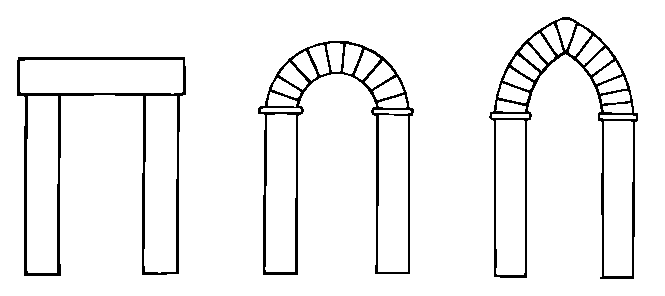
\includegraphics[width=0.85\linewidth]{images/motivacion/arcos.eps}
	\end{center}
\end{frame}

\begin{frame}[c]
	\frametitle{Motivación}
	\begin{center}
		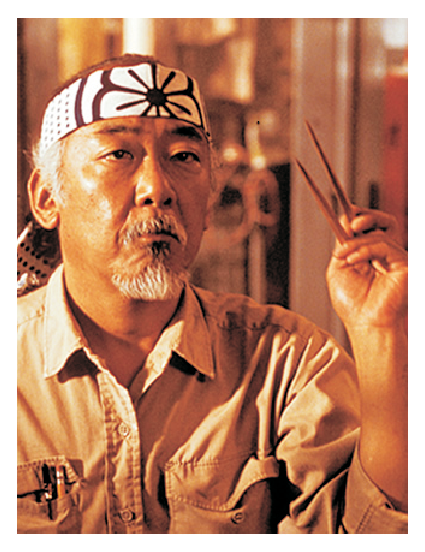
\includegraphics[width=0.45\linewidth]{images/motivacion/miyagi.eps}
	\end{center}
\end{frame}

\begin{frame}[c]
	\frametitle{Motivación}
	\begin{center}
		\textbf{Gol de Puyol a Alemania Sudáfrica 2010} \href{http://www.youtube.com/watch?v=Tnt7C2L6d3M}{(ver)}
	\end{center}
\end{frame}

\subsubsection{Definición de Patrón de Diseño Sw}

\begin{frame}[c]
	\frametitle{Patrón de Diseño Software}
	\begin{block}{Patrón de Diseño Software}
		\alert<2>{Solución probada y beneficiosa} a \alert<3>{problemas recurrentes} que aparecen continuamente durante el diseño de un producto software.
	\end{block}
	\uncover<4->{
	\begin{block}{Patrón de Diseño Software (Gamma et al, 1994)}
		Una descripción de cómo interconectar clases y objetos de forma que puedan resolver un problema general de diseño dentro de un contexto determinado.
	\end{block}
	}
\end{frame}

\begin{frame}[c]
	\frametitle{Estructura de un Patrón}
	\begin{enumerate}
		\item<+-> Nombre (y alias).
		\item<+-> Clasificación.
		\item<+-> Propósito.
		\item<+-> Motivación.
		\item<+-> Aplicabilidad.
		\item<+-> Estructura.
		\item<+-> Participantes.
		\item<+-> Interacción entre participantes.
		\item<+-> Consecuencias.
		\item<+-> Implementación.
		\item<+-> Ejemplos con código.
		\item<+-> Usos conocidos.
		\item<+-> Patrones relacionados.
	\end{enumerate}
\end{frame}

\begin{frame}[c]
	\frametitle{Tipos de Patrón}
	\begin{description}
		\item<+->[Creacionales] Relativos a problemas relacionados con la creación de objetos (ej. Factoría).
		\item<+->[Estructurales] Relativos a problemas relacionados con las relaciones y dependencias estáticas entre clases y objetos (ej. Peso mosca).
		\item<+->[De comportamiento] Relativos a problemas relacionados el comportamiento de clases y objetos en tiempo de ejecución (ej. Estrategia).
	\end{description}
\end{frame}

\subsection{Refactorizaciones}

\begin{frame}[c]
	\frametitle{Refactorizaciones}
	\begin{block}{Refactorización}
	Proceso de cambio de un sistema software de forma que su comportamiento externo no se vea afectado pero que mejora su estructura interna.
	% (ej. atributos relacionados a clase).
	% Extraer datos de una dirección a una clase dirección
	\end{block}
\end{frame}

\begin{frame}[c]
	\frametitle{Esquema de una Refactorización}
	\begin{enumerate}
		\item<1-> Nombre.
		\item<2-> Síntomas (bad smells).
		\item<3-> Causas.
		\item<4-> Refactorizaciones propuestas.
		\item<5-> Beneficios esperados.
		\item<6-> Efectos colaterales y contraindicaciones.
	\end{enumerate}
\end{frame}

\begin{frame}[c]
	\frametitle{Code Smells}
    \begin{block}{Malos olores (\emph{(bad) code smells})}
		Indicios sobre potenciales problemas en el código (ej. código replicado, mismo método en varias subclases).
	  \end{block}
\end{frame}

\subsection{Antipatrones}

\begin{frame}[c]
	\frametitle{Antipatrón de Diseño Software}
	\begin{block}{Antipatrón Software}
        Un \emph{antipatrón} describe una solución que genera consecuencias negativas para el desarrollo de un proyecto pero que se aplica recurrentemente a determinados problema.
	\end{block}
\end{frame}

\begin{frame}[c]
	\frametitle{Utilidad de los Antipatrones}
	\begin{enumerate}[<+->]
        \item Asocian situaciones conflictivas a un \alert{conjunto de soluciones}.
        \item Identifican situaciones conflictivas recurrentes.
        \item Proporcionan un vocabulario estandarizado para dichas situaciones conflictivas.
        \item Empatía en el fallo.
	\end{enumerate}
\end{frame}

\begin{frame}[c]
	\frametitle{Origen de los Antipatrones}
    \begin{enumerate}[<+->]
        \item Prisas.     % Mala calidad
        \item Apatía.     % Para qué
        \item Estrechez de miras. % No utilizar nuevas y probadas soluciones
        \item Pereza.     % Confiar en ya se hará con la herramienta
        \item Avaricia.   % Sistema excesivamente complejo
        \item Ignorancia. % Pereza intelectual.
        \item Orgullo.    % stdio está mal.
    \end{enumerate}
\end{frame}

%\begin{frame}[c]
%	\frametitle{Esquema de un Antipatrón}
%	\begin{enumerate}
%		\item<1-> Nombre.
%		\item<2-> Síntomas.
%		\item<3-> Causas.
%		\item<4-> Refactorizaciones propuestas.
%		\item<5-> Beneficios esperados.
%		\item<6-> Efectos colaterales y contraindicaciones.
%	\end{enumerate}
%\end{frame}

\subsection{Relación entre Patrones, Refactorizaciones y Antipatrones}

\begin{frame}[t]
	\frametitle{Patrones, Refactorizaciones y Antipatrones}
    \only<1>{
    \rput[lt](0,-1.5){
        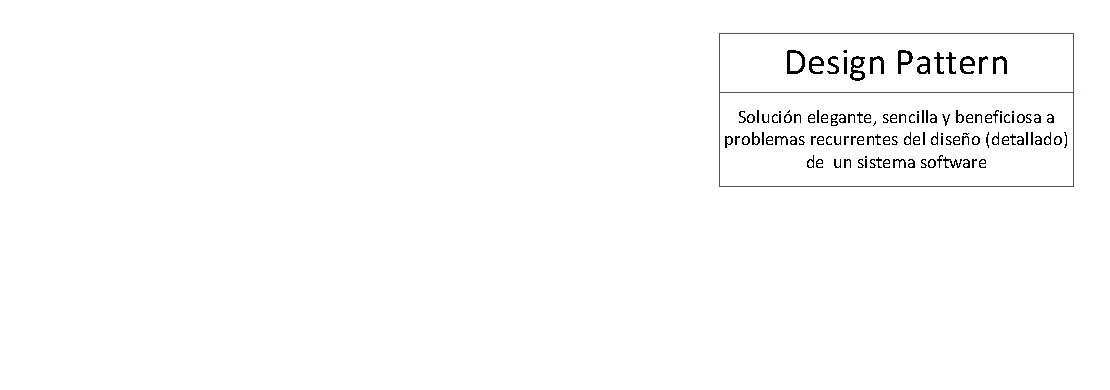
\includegraphics[width=11cm,keepaspectratio=true]{images/antipatterns/antipatternSchema00.eps}}}
    \only<2>{
    \rput[lt](0,-1.5){
        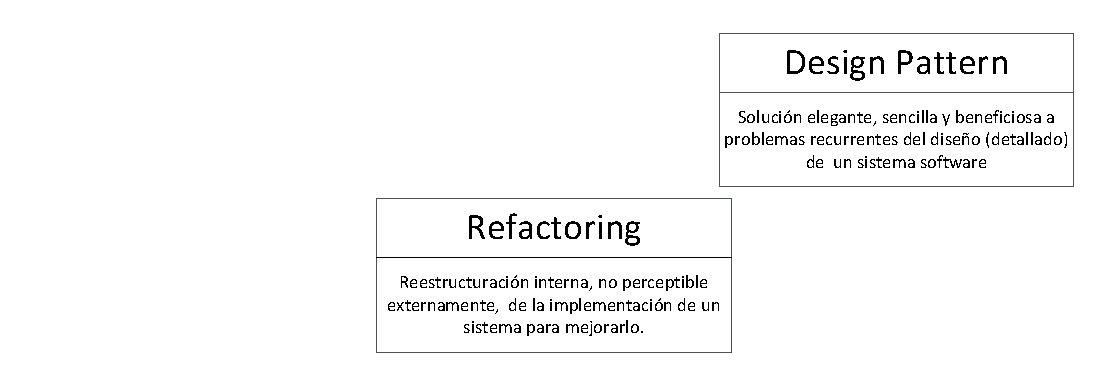
\includegraphics[width=11cm,keepaspectratio=true]{images/antipatterns/antipatternSchema01.eps}}}
    \only<3>{
    \rput[lt](0,-1.5){
        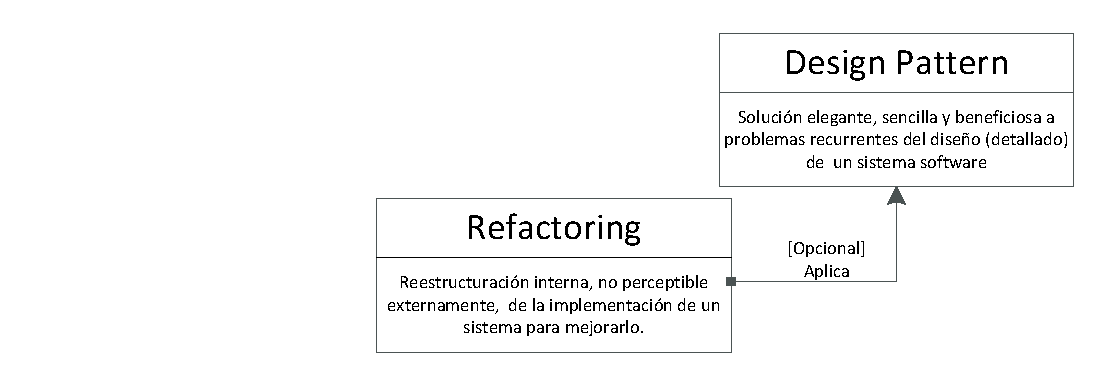
\includegraphics[width=11cm,keepaspectratio=true]{images/antipatterns/antipatternSchema02.eps}}}
    \only<4>{
    \rput[lt](0,-1.5){
        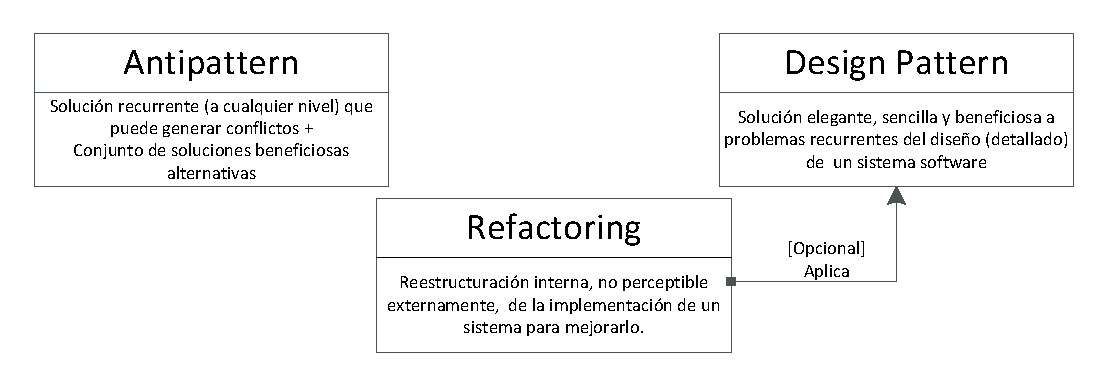
\includegraphics[width=11cm,keepaspectratio=true]{images/antipatterns/antipatternSchema03.eps}}}
    \only<5>{
    \rput[lt](0,-1.5){
        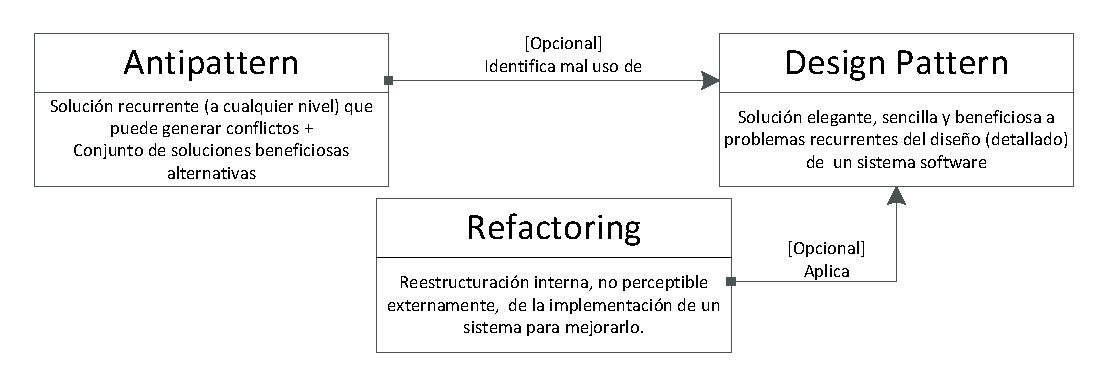
\includegraphics[width=11cm,keepaspectratio=true]{images/antipatterns/antipatternSchema04.eps}}}
    \only<6>{
    \rput[lt](0,-1.5){
        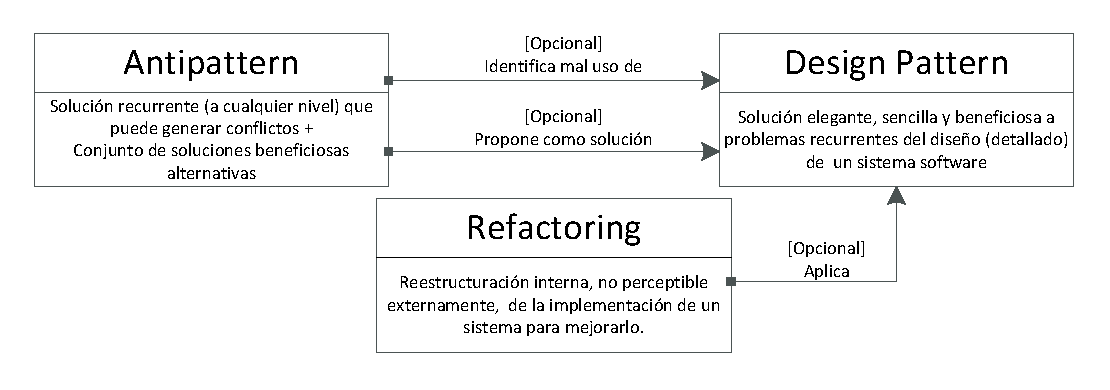
\includegraphics[width=11cm,keepaspectratio=true]{images/antipatterns/antipatternSchema05.eps}}}
    \only<7>{
    \rput[lt](0,-1.5){
        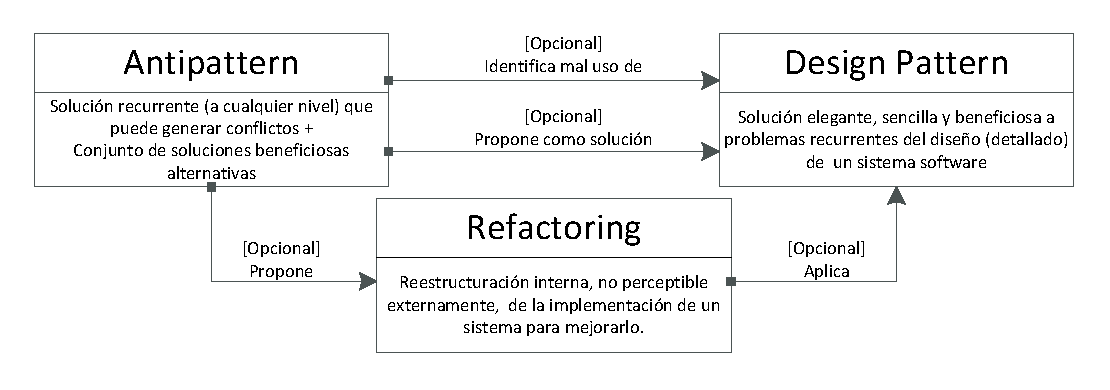
\includegraphics[width=11cm,keepaspectratio=true]{images/antipatterns/antipatternSchema06.eps}}}
\end{frame}

\section{Patrones de Diseño GoF}

\begin{frame}[c]
	\frametitle{Patrones GoF (Gang of Four) I}
	\begin{enumerate}
		\item Composite.
		\item Interpreter.
		\item Visitor.
		\item Strategy.
		\item Template Method.
        \item Singleton.
        \item Factory Method.
        \item Abstract Factory.
        \item Prototype.
	\end{enumerate}
\end{frame}

\begin{frame}[c]
	\frametitle{Patrones GoF (Gang of Four) II}
	\begin{enumerate}
        \item Observer
        \item Iterator.
        \item Proxy.
        \item Adapter.
        \item State.
	\end{enumerate}
\end{frame}

\begin{frame}[c]
	\frametitle{Patrones No GoF}
	\begin{enumerate}
		\item Mixin.
        \item Null Object.
		\item Pool Object.
        \item Type.
	\end{enumerate}
\end{frame}

%\frame[c]{
%	\frametitle{Índice}
%	\begin{enumerate}
%		\item Introducción.
%		\item Concepto de Patrón.
%		\item \alert{Patrones de diseño GoF}.
%		\item Otros patrones de diseño.
%		\item Antipatrones.
%		\item Refactorizaciones.
%		\item Sumario.
%	\end{enumerate}
%}
%
%\begin{frame}[c]
%	\frametitle{Patrones GoF (Gang of Four)}
%	\begin{enumerate}
%		\item \alert<2->{Singleton}.
%		\item Factoría abstracta.
%		\item Adaptador.
%		\item Estrategia.
%		\item Estado.
%	\end{enumerate}
%\end{frame}
%
%\subsection{Singleton}
%
%\begin{frame}[c]
%	\frametitle{Patrón Singleton}
%	\begin{block}{Problema}
%		Sólo debe existir una instancia de una clase (ej. driver de ratón).
%	\end{block}
%	\uncover<2->{
%	\begin{block}{Aplicabilidad}
%		Sólo debe existir una instancia por clase, la cual debe estar accesible desde un punto de entrada bien definido.
%	\end{block}
%	}
%\end{frame}
%
%\begin{frame}[c]
%	\frametitle{Patrón Singleton}
%	\begin{center}
%		\includegraphics[width=\linewidth,keepaspectratio=true]{images/gof/singleton00.eps}
%	\end{center}
%\end{frame}
%
% \subsection{Factoría Abstracta}
%
%\begin{frame}[c]
%	\frametitle{Patrones GoF (Gang of Four)}
%	\begin{enumerate}
%		\item Singleton.
%		\item \alert{Factoría abstracta}.
%		\item Adaptador.
%		\item Estrategia.
%		\item Estado.
%	\end{enumerate}
%\end{frame}
%
%\begin{frame}[c]
%	\frametitle{Patrón Factoría Abstracta}
%	\begin{block}{Problema}
%		Dependencia de clases concretas. \\
%		\uncover<2->{Ej. \texttt{List<Persona> listaAsistentes = new ArrayList<Persona>}}
%	\end{block}
%\end{frame}
%
%\begin{frame}[c]
%	\frametitle{Patrón Factoría Abstracta - Problema}
%	\begin{center}
%		\includegraphics[width=\linewidth,keepaspectratio=true]{images/gof/abstractFactory00.eps}
%	\end{center}
%\end{frame}
%
%\begin{frame}[c]
%	\frametitle{Patrón Factoría Abstracta}
%	\begin{block}{Aplicabilidad}
%		\begin{enumerate}
%			\item<+-> Un sistema debe ser independiente de como sus productos son creados, compuestos y representados.
%			\item<+-> Un sistema debe ser configurado usando un conjunto coherente de clases concretas.
%			\item<+-> Deseamos crear una librería de productos, pero sólo queremos hacer públicas las interfaces, no las implementaciones.
%		\end{enumerate}
%	\end{block}
%\end{frame}
%
%\begin{frame}[c]
%	\frametitle{Patrón Factoría Abstracta - Solución}
%	\begin{center}
%		\includegraphics[width=\linewidth,keepaspectratio=true]{images/gof/abstractFactory01.eps}
%	\end{center}
%\end{frame}
%
%\begin{frame}[c]
%	\frametitle{Patrón Factoría Abstracta}
%	\begin{center}\textbf{Ventajas}\end{center}
%	\begin{enumerate}
%		\item<+-> Hace independientes las clases clientes de clases concretas particulares.
%		\item<+-> Hace más fácil cambiar la configuración actual de un producto, ya que sólo hay que cambiar la factoría concreta.
%		\item<+-> Favorece la consistencia entre productos.
%	\end{enumerate}
%\end{frame}
%
%\subsection{Adaptador}
%
%\begin{frame}[c]
%	\frametitle{Patrones GoF (Gang of Four)}
%	\begin{enumerate}
%		\item Singleton.
%		\item Factoría abstracta.
%		\item \alert{Adaptador}.
%		\item Estrategia.
%		\item Estado.
%	\end{enumerate}
%\end{frame}
%
%\begin{frame}[c]
%	\frametitle{Patrón Adaptador}
%	\begin{block}{Problema}
%		La interfaz de una clase no se corresponde con la interfaz esperada por los clientes.
%	\end{block}
%\end{frame}
%
%\begin{frame}[c]
%	\frametitle{Patrón Adaptador}
%	\begin{center}
%		\includegraphics[width=.85\linewidth,keepaspectratio=true]{images/gof/adapter00.eps}
%	\end{center}
%\end{frame}
%
%\begin{frame}[c]
%	\frametitle{Patrón Adaptador}
%	\begin{center}
%		\includegraphics[width=.9\linewidth,keepaspectratio=true]{images/gof/adapter01.eps}
%	\end{center}
%\end{frame}
%
%\begin{frame}[c]
%	\frametitle{Patrón Adaptador}
%	\begin{center}
%		\includegraphics[width=.9\linewidth,keepaspectratio=true]{images/gof/adapter02.eps}
%	\end{center}
%\end{frame}
%
%\subsection{Estrategia}
%
%\begin{frame}[c]
%	\frametitle{Patrones GoF (Gang of Four)}
%	\begin{enumerate}
%		\item Singleton.
%		\item Factoría abstracta.
%		\item Adaptador.
%		\item \alert{Estrategia}.
%		\item Estado.
%	\end{enumerate}
%\end{frame}
%
%\begin{frame}[c]
%	\frametitle{Patrón Estrategia}
%	\begin{block}{Problema}
%		La implementación de un método debe variar, pero queremos hacer a las clases clientes ignoren dicha cuestión.
%	\end{block}
%\end{frame}
%
%\begin{frame}[c]
%	\frametitle{Patrón Estrategia}
%	\begin{center}
%		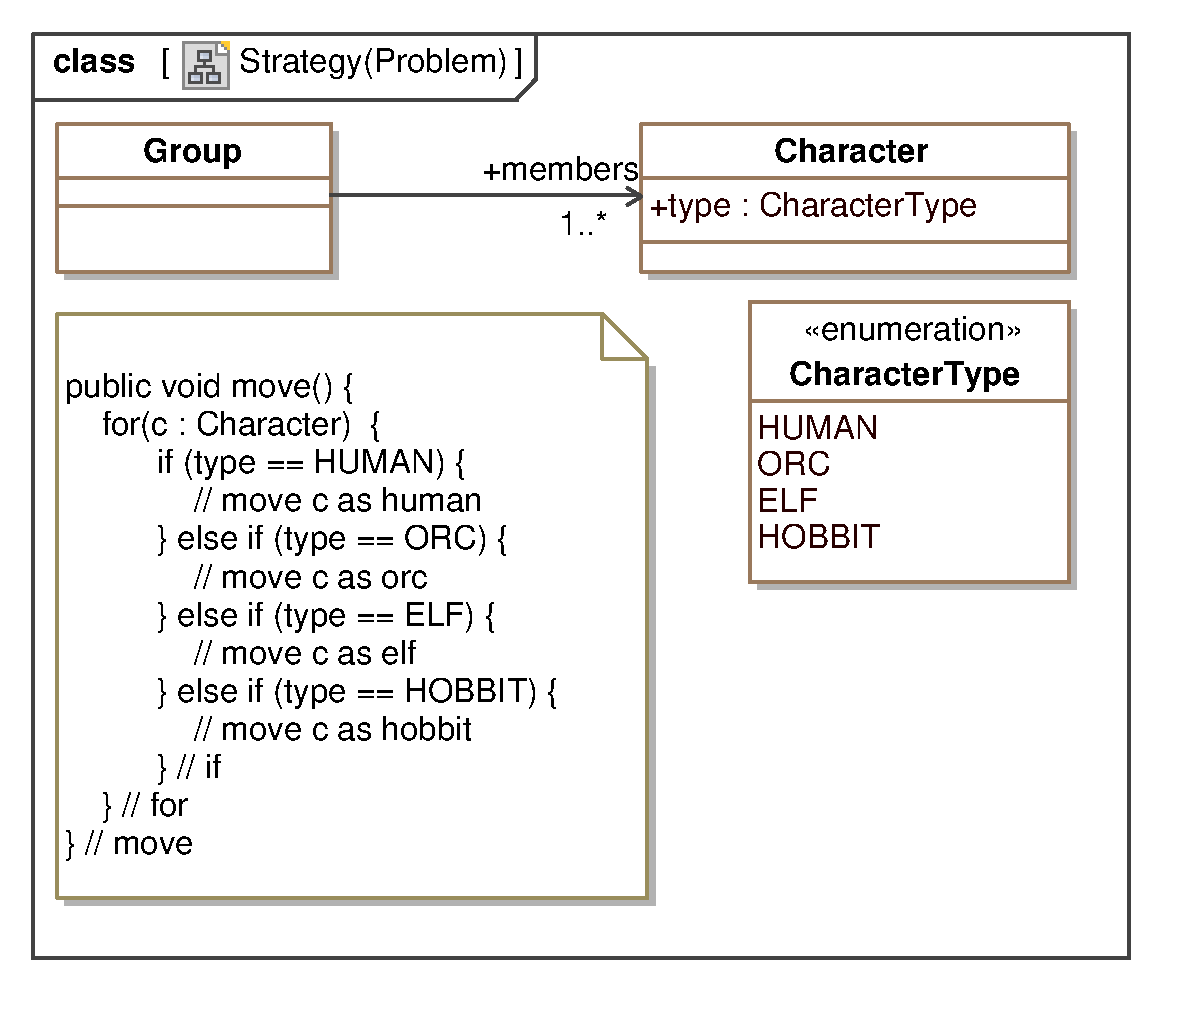
\includegraphics[width=.65\linewidth,keepaspectratio=true]{images/gof/Strategy00.eps}
%	\end{center}
%\end{frame}
%
%\begin{frame}[c]
%	\frametitle{Patrón Estrategia}
%	\begin{block}{Aplicación}
%		\begin{enumerate}
%			\item<+-> Varias clases sólo difieren en el comportamiento de una o dos responsabilidades
%			\item<+-> Es necesario implementar diversas variantes de un mismo algoritmo y seleccionar una variante concreta en tiempo de ejecución.
%		\end{enumerate}
%	\end{block}
%\end{frame}
%
%\begin{frame}[c]
%	\frametitle{Patrón Estrategia}
%	\begin{center}
%		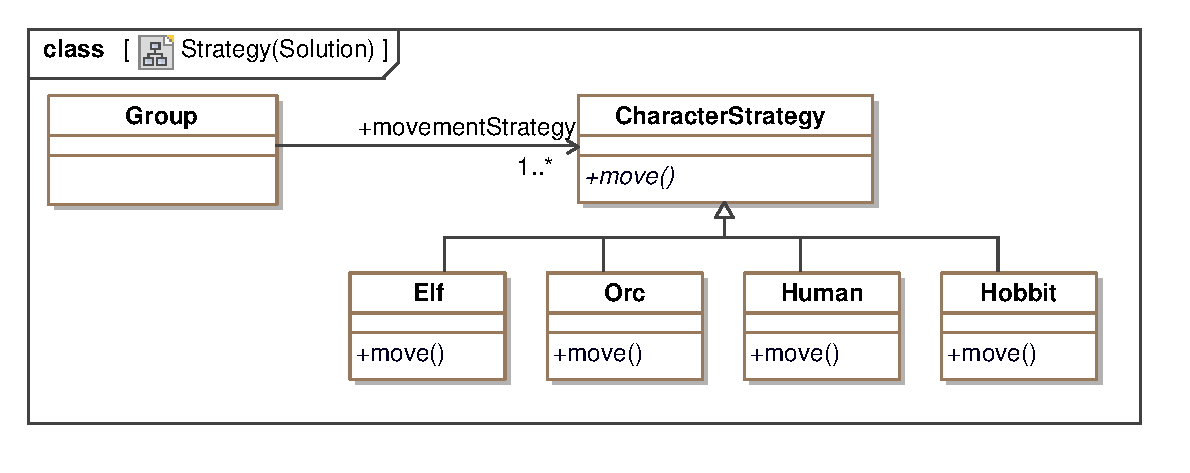
\includegraphics[width=.9\linewidth,keepaspectratio=true]{images/gof/Strategy01.eps}
%	\end{center}
%\end{frame}
%
%\subsection{Estado}
%
%\begin{frame}[c]
%	\frametitle{Patrones GoF (Gang of Four)}
%	\begin{enumerate}
%		\item Singleton.
%		\item Factoría abstracta.
%		\item Adaptador (Wrapper).
%		\item Estrategia.
%		\item \alert{Estado}.
%	\end{enumerate}
%\end{frame}
%
%\begin{frame}[c]
%	\frametitle{Patrón Estado}
%	\begin{block}{Problema}
%		Un objeto necesita variar su comportamiento cuando cambia de estado.
%	\end{block}
%\end{frame}
%
%\begin{frame}[c]
%	\frametitle{Patrón Estado}
%	\begin{center}
%		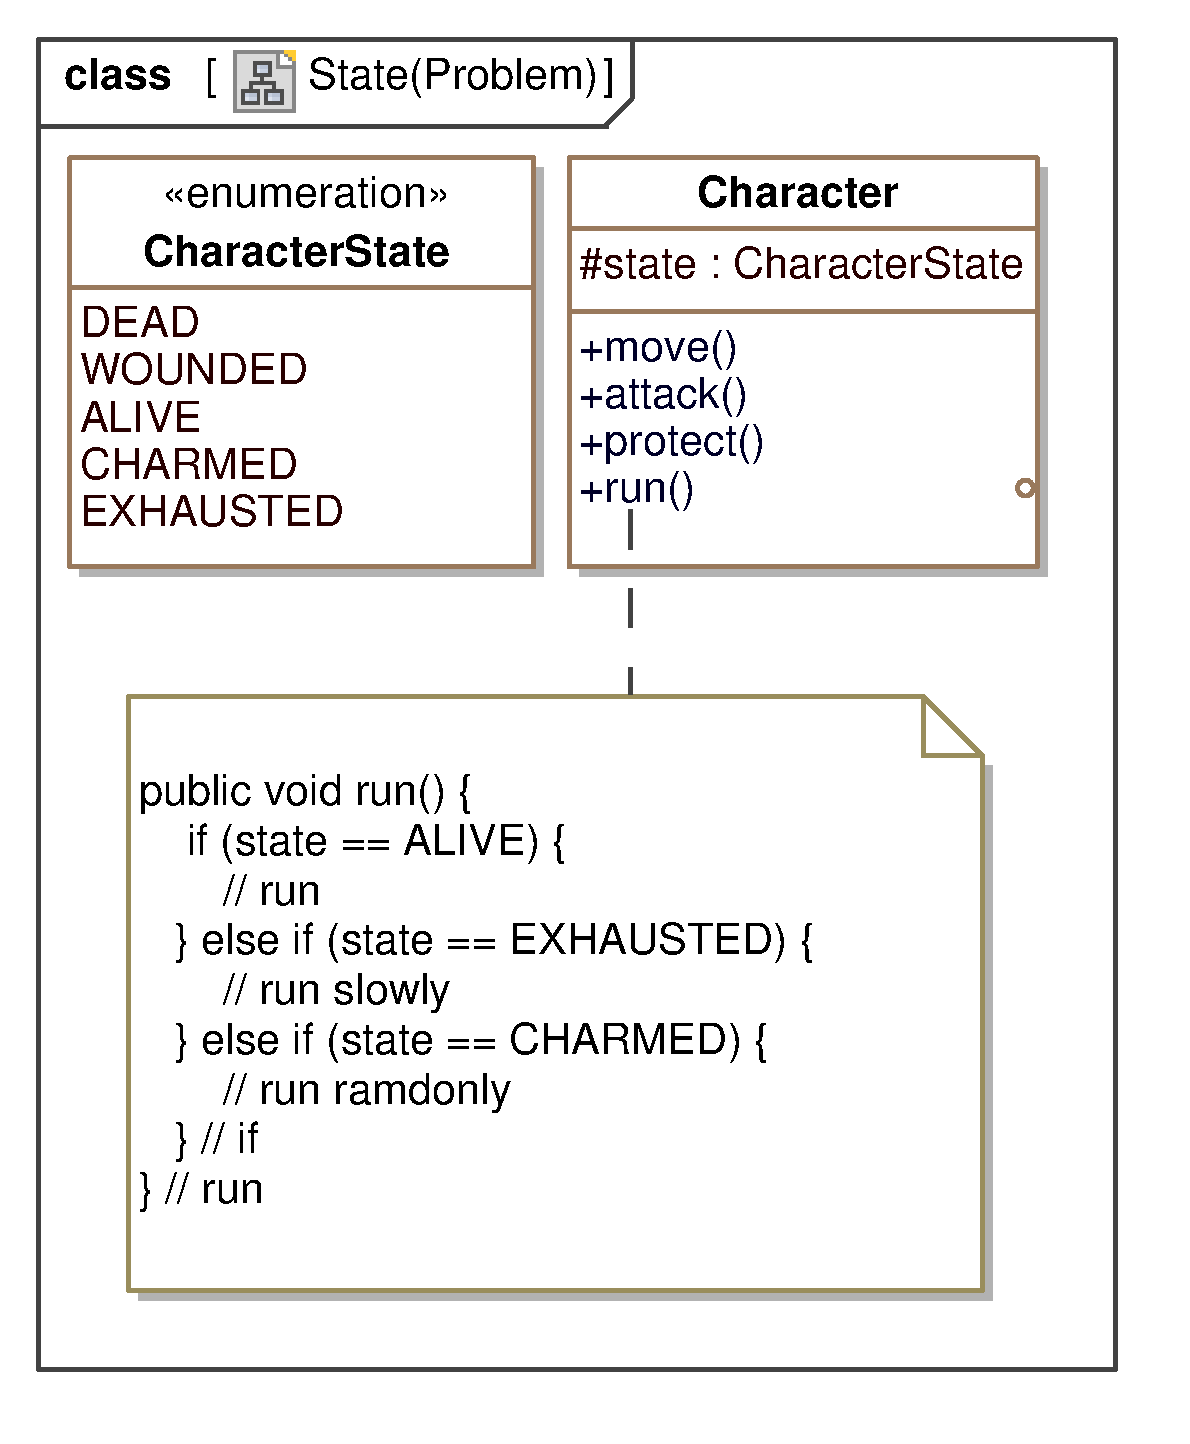
\includegraphics[width=.50\linewidth,keepaspectratio=true]{images/gof/State00.eps}
%	\end{center}
%\end{frame}
%
%\begin{frame}[c]
%	\frametitle{Patrón Estado}
%	\begin{center}
%		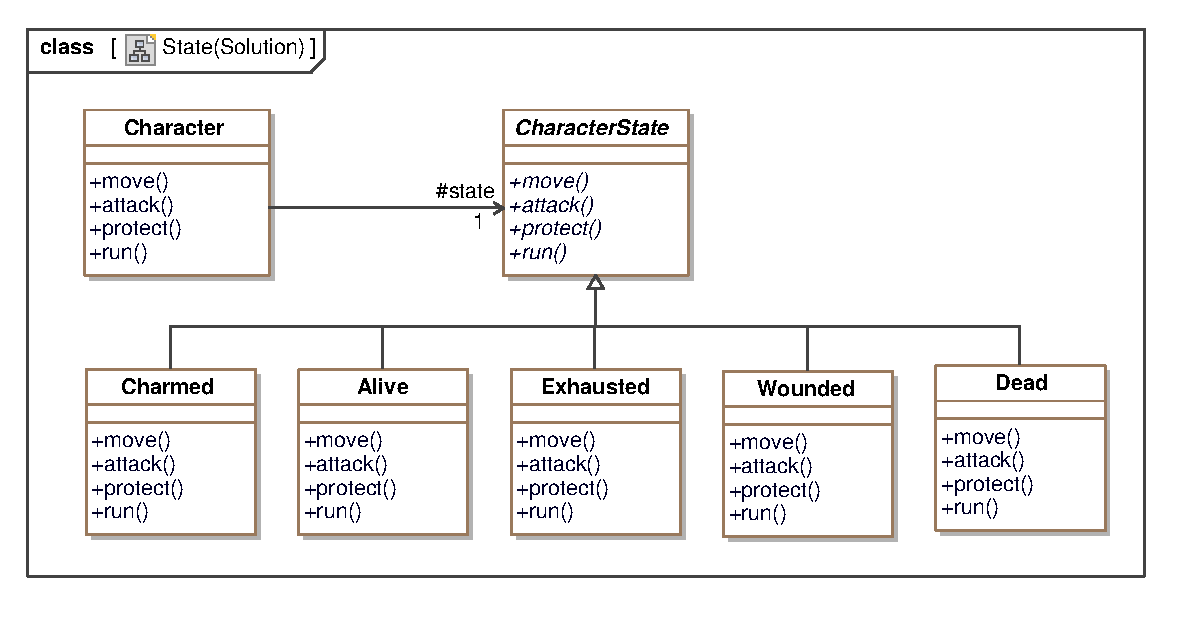
\includegraphics[width=\linewidth,keepaspectratio=true]{images/gof/State01.eps}
%	\end{center}
%\end{frame}
%
%\section{Otros Patrones de Diseño}
%
%\frame[c]{
%	\frametitle{Índice}
%	\begin{enumerate}
%		\item Introducción.
%		\item Concepto de Patrón.
%		\item Patrones de diseño GoF.
%		\item \alert{Otros patrones de diseño}.
%		\item Antipatrones.
%		\item Refactorizaciones.
%		\item Sumario.
%	\end{enumerate}
%}
%
%\frame[c]{
%	\frametitle{Patrones de Diseño no GoF}
%	\begin{enumerate}
%		\item \alert<2->{Patrón Tipo}.
%		\item Patrón \emph{Mixin}.
%	\end{enumerate}
%}
%
%\subsection{Patrón Tipo}
%
%\begin{frame}[c]
%	\frametitle{Patrón Tipo}
%	\begin{block}{Aplicación}
%		\begin{enumerate}
%			\item Permitir que un objeto pueda cambiar su(s) tipo(s) de forma dinámica en tiempo de ejecución.
%			\item Permitir que se puedan crear nuevos tipos de forma dinámica en tiempo de ejecución.
%		\end{enumerate}
%	\end{block}
%\end{frame}
%
%\begin{frame}[c]
%	\frametitle{Patrón Tipo}
%	\begin{center}
%		\includegraphics[width=\linewidth,keepaspectratio=true]{images/nogof/type00.eps}
%	\end{center}
%\end{frame}
%
%\begin{frame}[c]
%	\frametitle{Patrón Tipo}
%	\begin{center}
%		\includegraphics[width=.65\linewidth,keepaspectratio=true]{images/nogof/type01.eps}
%	\end{center}
%\end{frame}
%
%\subsection{Patrón Mixin}
%
%\frame[c]{
%	\frametitle{Patrones de Diseño no GoF}
%	\begin{enumerate}
%		\item Patrón Tipo.
%		\item \alert{Patrón \emph{Mixin}}.
%	\end{enumerate}
%}
%
%\begin{frame}[c]
%	\frametitle{Patrón Mixin}
%	\begin{block}{Aplicación}
%		Permitir herencia múltiple en lenguajes que no permiten herencia múltiple de clases, pero si de interfaces.
%	\end{block}
%\end{frame}
%
%\begin{frame}[t]
%	\frametitle{Patrón Mixin}
%	\begin{center}
%		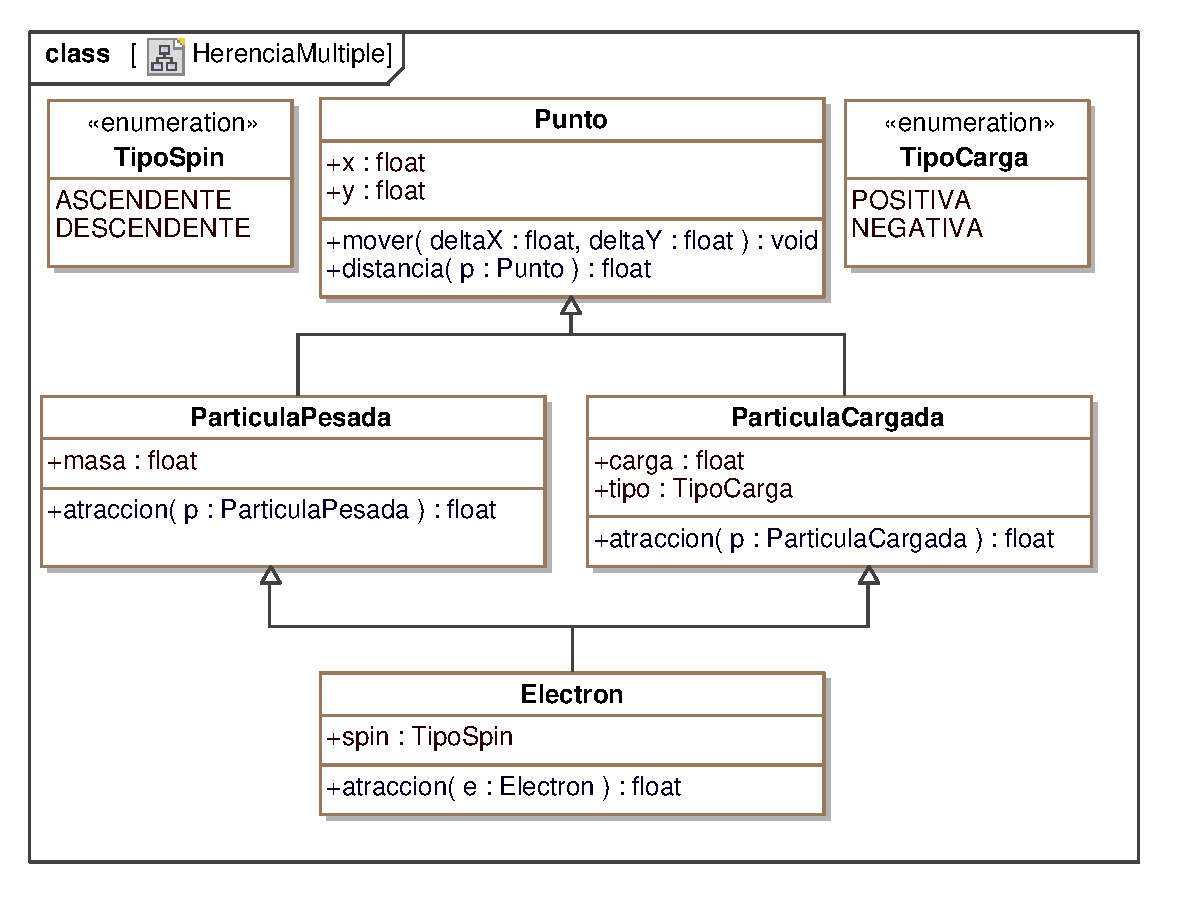
\includegraphics[clip=true,width=.75\linewidth]{images/nogof/Mixin00.eps}
%	\end{center}
%\end{frame}
%
%\begin{frame}[t]
%	\frametitle{Patrón Mixin}
%	\begin{center}
%		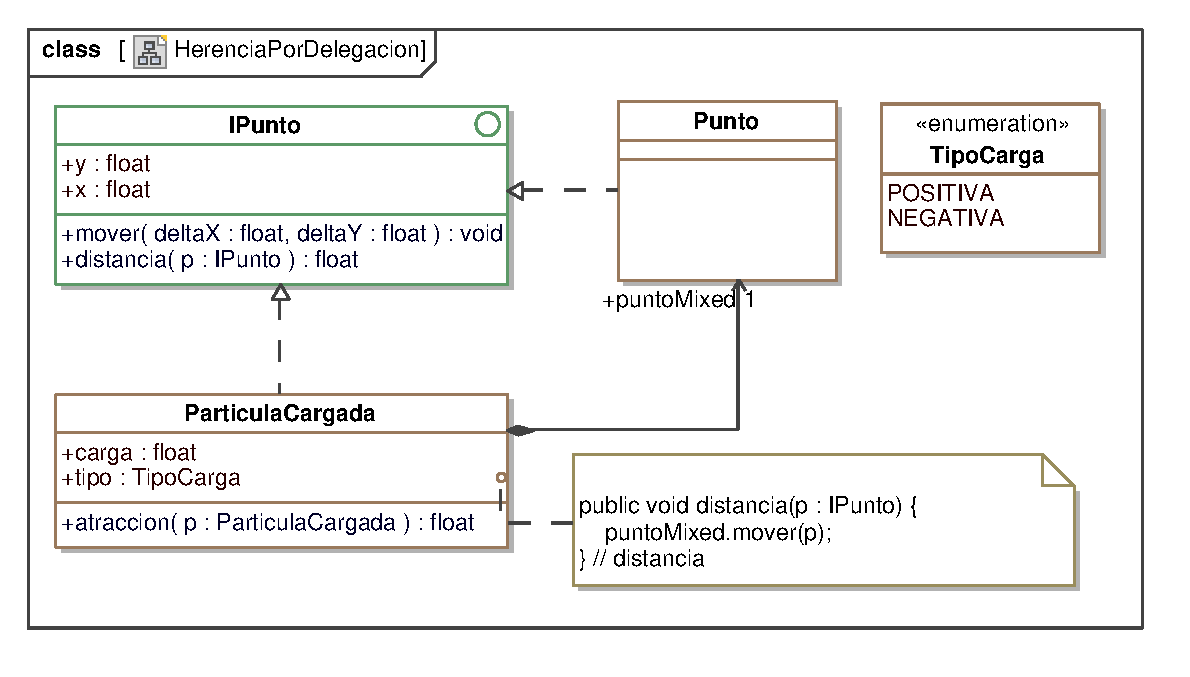
\includegraphics[clip=true,width=0.9\linewidth]{images/nogof/Mixin01.eps}
%	\end{center}
%\end{frame}
%
%\begin{frame}[t]
%	\frametitle{Patrón Mixin}
%	\begin{center}
%		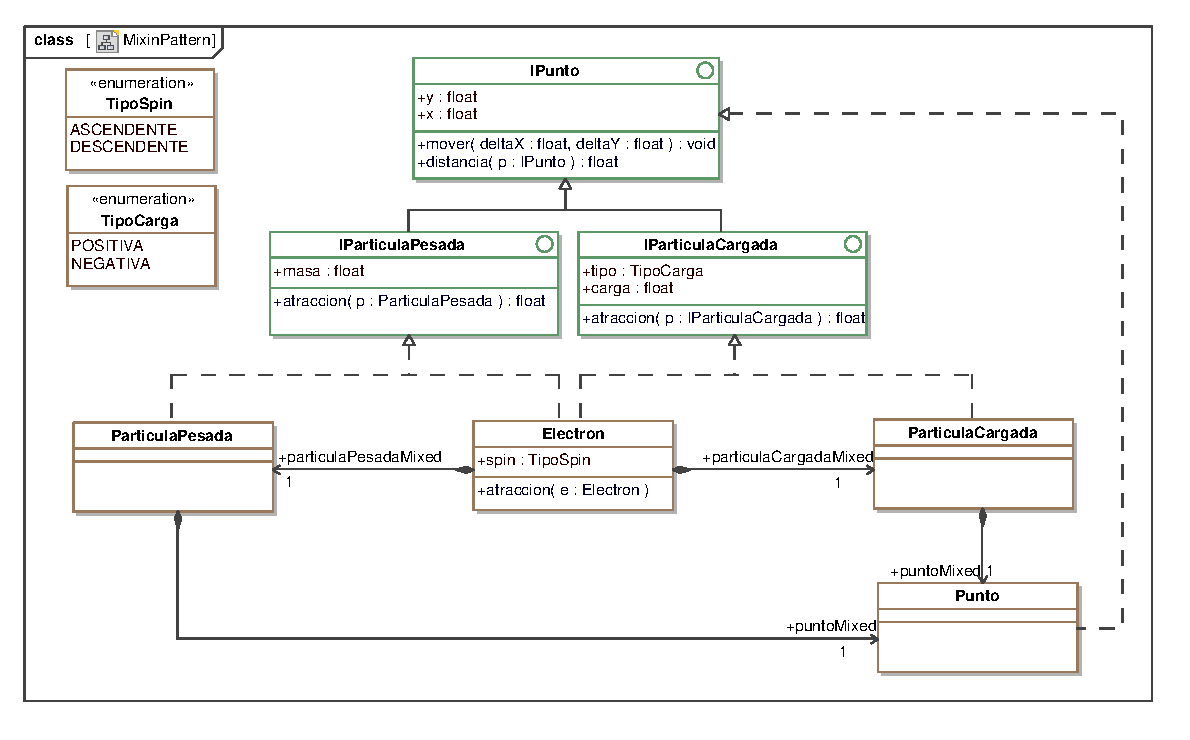
\includegraphics[clip=true,width=\linewidth]{images/nogof/Mixin02.eps}
%	\end{center}
%\end{frame}

\section{Refactorizaciones}

%\subsection{Introducción}
%
%\begin{frame}[t]
%	\frametitle{Refactorizaciones}
%	\begin{block}{Refactorización}
%	Proceso de cambio de un sistema software de forma que su comportamiento externo no se vea afectado pero que mejora su estructura interna.
%	% (ej. atributos relacionados a clase).
%	% Extraer datos de una dirección a una clase dirección
%	\end{block}
%	\uncover<2->{
%		\begin{block}{Malos olores (bad smells)}
%		Indicios sobre potenciales problemas en el código (ej. código replicado, mismo método en varias subclases).
%		\end{block}
%	}
%\end{frame}
%
%\begin{frame}[c]
%	\frametitle{Esquema de una Refactorización}
%	\begin{enumerate}
%		\item<1-> Nombre
%		\item<2-> Síntomas
%		\item<3-> Causas
%		\item<4-> Refactorizaciones propuestas
%		\item<5-> Beneficios esperados
%		\item<6-> Efectos colaterales y contraindicaciones
%	\end{enumerate}
%\end{frame}

\begin{frame}[c]
	\frametitle{Refactorizaciones más Populares~\cite{counsell:2006}}
	\begin{enumerate}
		\item Pull Up Method.
		\item Move Method.
		\item Introduce Parameter Object.
		\item Move Field.
		\item Rename Method/Field.
		\item Replace Magic Number with Symbolic Constant.
		\item Replace Type Code with State/Strategy.
	\end{enumerate}
\end{frame}

\subsection{Pull Up Method}

\begin{frame}
	\frametitle{Pull Up Method}
	\begin{block}{Descripción}
		Existen métodos \emph{cuasi}-idénticos en las subclases
	\end{block}
	\begin{columns}
		\column{.50\linewidth}
		\begin{center}
			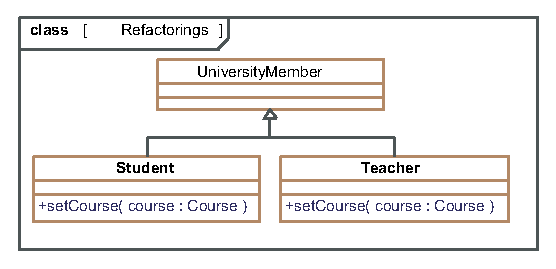
\includegraphics[width=\textwidth,keepaspectratio=true]{images/refactorings/pum00.eps}
		\end{center}
		\column{.10\linewidth}
			\ \\
			\ \\
			\ \\
			\Huge $\Rightarrow$
		\column{.40\linewidth}
		\only<2->{
		\begin{center}
			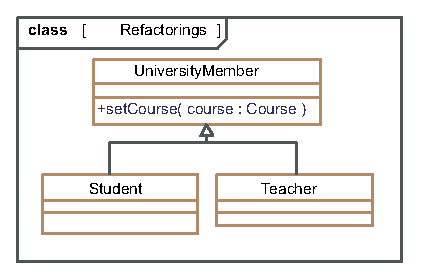
\includegraphics[width=\textwidth,keepaspectratio=true]{images/refactorings/pum01.eps}
		\end{center}
		}
	\end{columns}
\end{frame}

\subsection{Move Method}

\begin{frame}
	\frametitle{Move Method}
	\begin{block}{Descripción}
		Un método de una clase A es más utilizado en una clase B que en la clase A donde está definido.
	\end{block}
	\begin{columns}
		\column{.45\linewidth}
		\begin{center}
			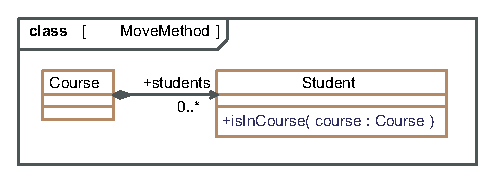
\includegraphics[width=\textwidth,keepaspectratio=true]{images/refactorings/mm00.eps}
		\end{center}
		\column{.10\linewidth}
		\begin{center}
			\Huge $\Rightarrow$
		\end{center}
		\column{.45\linewidth}
		\only<2->{
		\begin{center}
			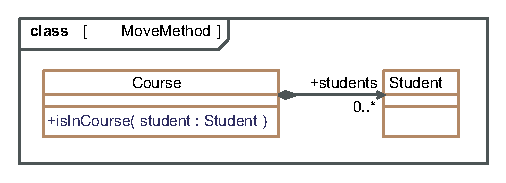
\includegraphics[width=\textwidth,keepaspectratio=true]{images/refactorings/mm01.eps}
		\end{center}
		}
	\end{columns}
\end{frame}

\subsection{Introduce Parameter Object}

%\begin{frame}
%    \frametitle{Add Parameter}
%    \begin{block}{Descripción}
%        Un método precisa conocer más información cuando es invocado por los clientes de una clase.
%    \end{block}
%    \begin{columns}
%        \column{.45\linewidth}
%        \begin{center}
%            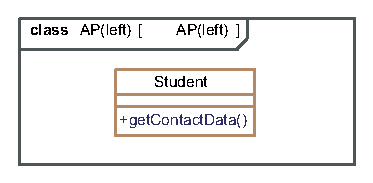
\includegraphics[width=.9\textwidth,keepaspectratio=true]{images/refactorings/ap00.eps}
%        \end{center}
%        \column{.10\linewidth}
%        \begin{center}
%            \ \\
%            \Huge $\Rightarrow$
%        \end{center}
%        \column{.45\linewidth}
%        \only<2->{
%        \begin{center}
%            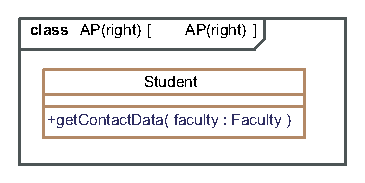
\includegraphics[width=.9\textwidth,keepaspectratio=true]{images/refactorings/ap01.eps}
%        \end{center}
%        }
%    \end{columns}
%    \ \\
%    \ \\
%    \only<3->{
%    \begin{center}
%        \textbf{¡ OJO !} puede crear listas interminables de argumentos
%    \end{center}}
%\end{frame}

\begin{frame}
	\frametitle{Introduce Parameter Object}
	\begin{block}{Descripción}
		% You have a group of parameters that naturally go together.
		Existen grupos de parámetros que están naturalmente relacionados
	\end{block}
	\begin{columns}
		\column{.45\linewidth}
		\begin{center}
			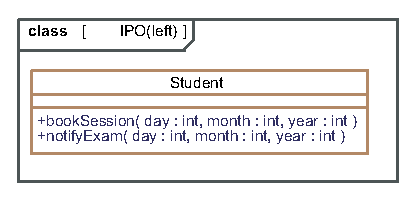
\includegraphics[width=.9\textwidth,keepaspectratio=true]{images/refactorings/ipo00.eps}
		\end{center}
		\column{.10\linewidth}
		\begin{center}
			\Huge $\Rightarrow$
		\end{center}
		\column{.45\linewidth}
		\only<2->{
		\begin{center}
			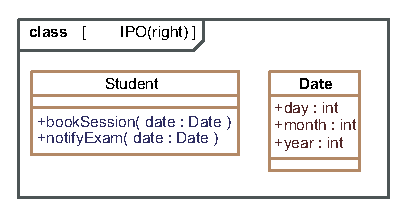
\includegraphics[width=.9\textwidth,keepaspectratio=true]{images/refactorings/ipo01.eps}
		\end{center}
		}
	\end{columns}
\end{frame}

\subsection{Move Field}

\begin{frame}
	\frametitle{Move Field}
	\begin{block}{Descripción}
	Un atributo de una clase A es más utilizado en una clase B que en la clase A donde está definido.
	\end{block}
	\begin{columns}
		\column{.45\linewidth}
		\begin{center}
			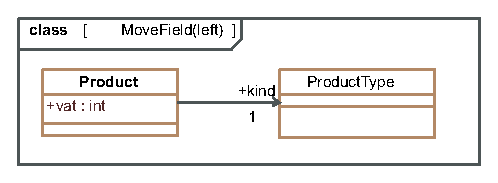
\includegraphics[width=\textwidth,keepaspectratio=true]{images/refactorings/mf00.eps}
		\end{center}
		\column{.10\linewidth}
		\begin{center}
			\Huge $\Rightarrow$
		\end{center}
		\column{.45\linewidth}
		\only<2->{
		\begin{center}
			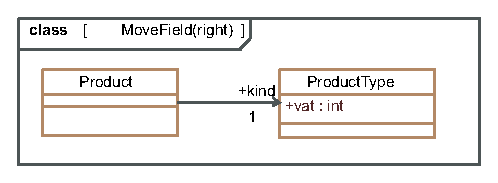
\includegraphics[width=\textwidth,keepaspectratio=true]{images/refactorings/mf01.eps}
		\end{center}
		}
	\end{columns}
\end{frame}

\subsection{Rename Method/Field}

\begin{frame}
	\frametitle{Rename Field/Method}
	\begin{block}{Descripción}
	% The name of a method does not reveal its purpose.
	El nombre de un atributo o método no es significativo
	\end{block}
	\begin{columns}
		\column{.45\linewidth}
		\begin{center}
			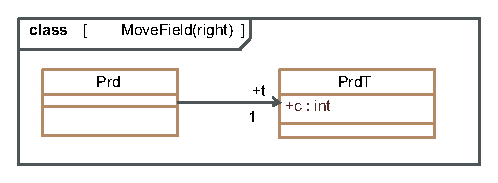
\includegraphics[width=\textwidth,keepaspectratio=true]{images/refactorings/rmf00.eps}
		\end{center}
		\column{.10\linewidth}
		\begin{center}
			\Huge $\Rightarrow$
		\end{center}
		\column{.45\linewidth}
		\only<2->{
		\begin{center}
			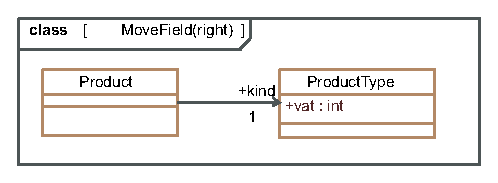
\includegraphics[width=\textwidth,keepaspectratio=true]{images/refactorings/mf01.eps}
		\end{center}
		}
	\end{columns}
\end{frame}

\subsection{Replace Magic Number}

\begin{frame}[fragile]
	\frametitle{Replace Magic Number with Symbolic Constant}
	\begin{block}{Descripción}
	% The name of a method does not reveal its purpose.
	Tenemos una constante numérica con un significado bien definido
	\end{block}
	\begin{scriptsize}
	\begin{semiverbatim}
	double calculateTotalCharge() \{
	   return this.totalAmount +
			 (this.totalAmount*16.0/100.0);
	\}
	\end{semiverbatim}
	\end{scriptsize}
	\begin{center}
		\textbf{refactors to}
	\end{center}
	\begin{scriptsize}
	\begin{semiverbatim}
	static final double NORMAL_VAT = 16.0;

	double calculateTotalCharge() \{
	   return this.totalAmount +
			 (this.totalAmount*NORMAL_VAT/100.0);
	\}
	\end{semiverbatim}
	\end{scriptsize}
\end{frame}

\subsection{Replace Type Code}

\begin{frame}[fragile]
	\frametitle{Replace Type Code with State/Strategy}
	\begin{block}{Descripción}
		Una clase tiene un atributo que indica tipo y que afecta al comportamiento de la clase
	\end{block}
	\begin{columns}
		\column{.40\linewidth}
		\begin{center}
			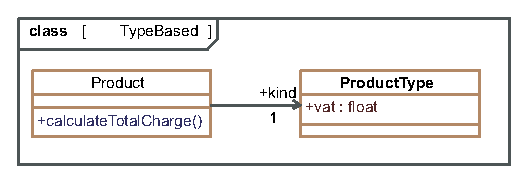
\includegraphics[width=\textwidth,keepaspectratio=true]{images/refactorings/strategy00.eps}
		\end{center}
		\column{.05\linewidth}
			\ \\
			\ \\
			\Huge $\Rightarrow$
		\column{.50\linewidth}
		\only<2->{
		\begin{center}
			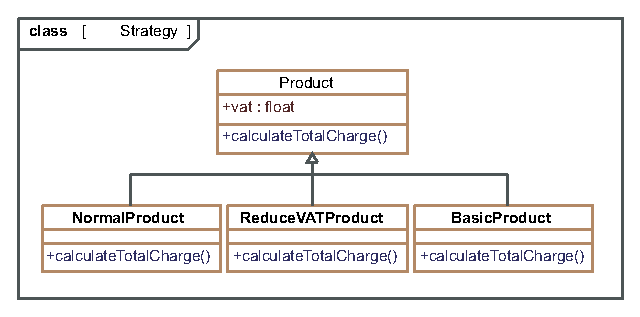
\includegraphics[width=\textwidth,keepaspectratio=true]{images/refactorings/strategy01.eps}
		\end{center}
		}
	\end{columns}
\end{frame}

\section{Antipatrones}

%\subsection{Concepto de Antipatrón}
%
%\begin{frame}[c]
%	\frametitle{Antipatrón de Diseño Software}
%	\begin{block}{Antipatrón Software}
%        Un \emph{antipatrón} describe una solución que genera consecuencias negativas para el desarrollo de un proyecto pero que se aplica recurrentemente a determinados problema.
%	\end{block}
%\end{frame}
%
%%%\begin{frame}[c]
%%%	\frametitle{Utilidad de los Antipatrones}
%%%	\begin{enumerate}[<+->]
%%%        \item Asocian situaciones conflictivas a un \alert{conjunto de soluciones}.
%%%        \item Identifican situaciones conflictivas recurrentes.
%%%        \item Proporcionan un vocabulario estandarizado para dichas situaciones conflictivas.
%%%        \item Mal de muchos, consuelo de tontos.
%%%	\end{enumerate}
%%%\end{frame}
%
%\begin{frame}[t]
%	\frametitle{Antipatrones, Refactorizaciones y Patrones}
%    \only<1>{
%    \rput[lt](0,-1.5){
%        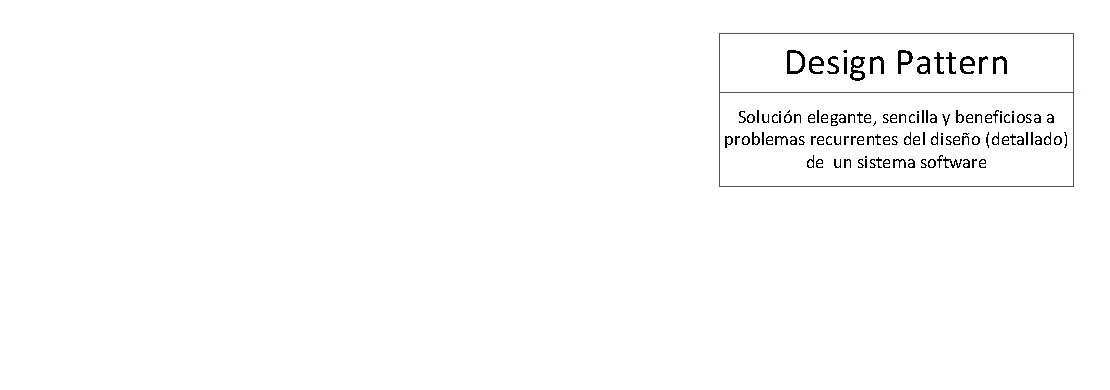
\includegraphics[width=11cm,keepaspectratio=true]{images/antipatterns/antipatternSchema00.eps}}}
%    \only<2>{
%    \rput[lt](0,-1.5){
%        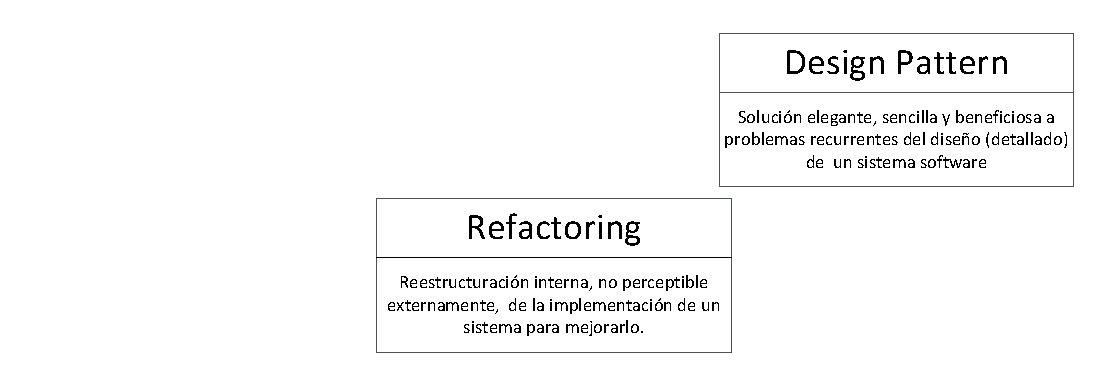
\includegraphics[width=11cm,keepaspectratio=true]{images/antipatterns/antipatternSchema01.eps}}}
%    \only<3>{
%    \rput[lt](0,-1.5){
%        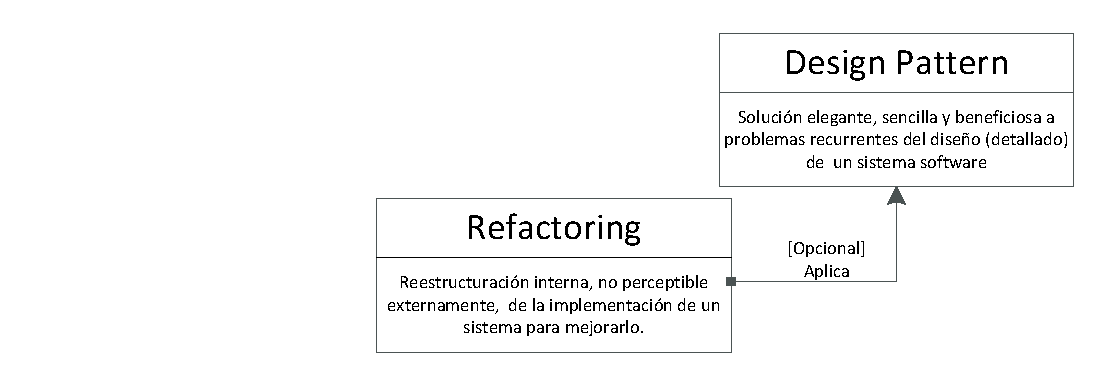
\includegraphics[width=11cm,keepaspectratio=true]{images/antipatterns/antipatternSchema02.eps}}}
%    \only<4>{
%    \rput[lt](0,-1.5){
%        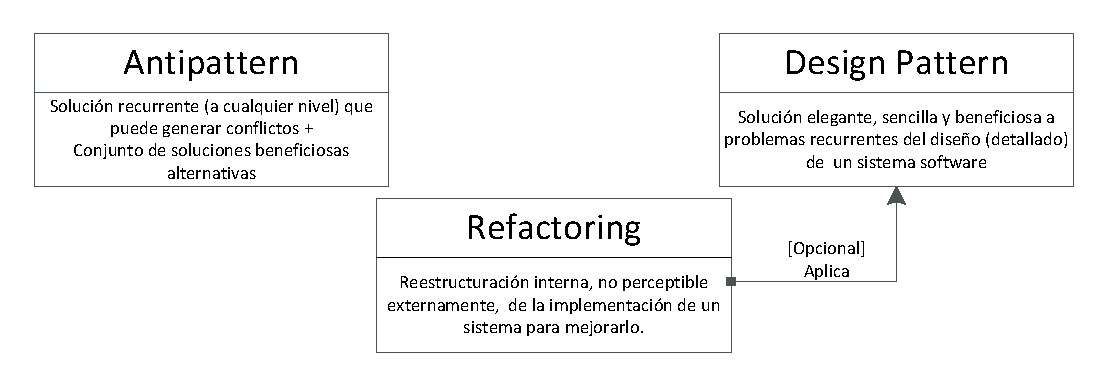
\includegraphics[width=11cm,keepaspectratio=true]{images/antipatterns/antipatternSchema03.eps}}}
%    \only<5>{
%    \rput[lt](0,-1.5){
%        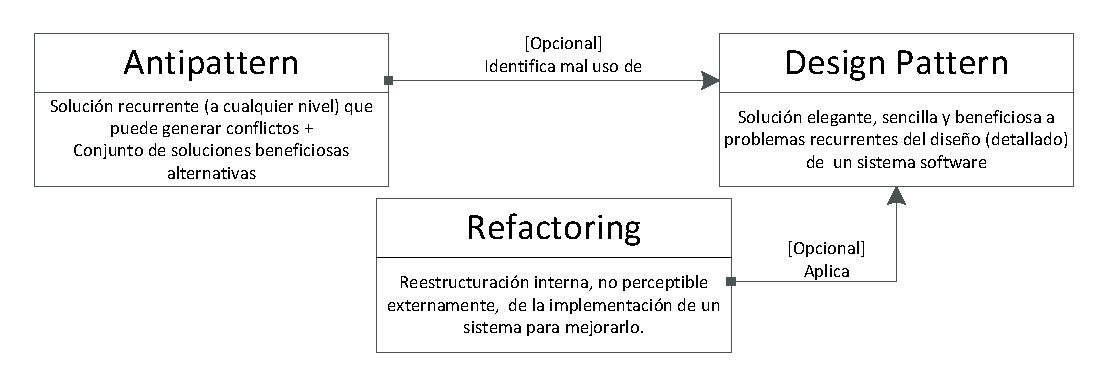
\includegraphics[width=11cm,keepaspectratio=true]{images/antipatterns/antipatternSchema04.eps}}}
%    \only<6>{
%    \rput[lt](0,-1.5){
%        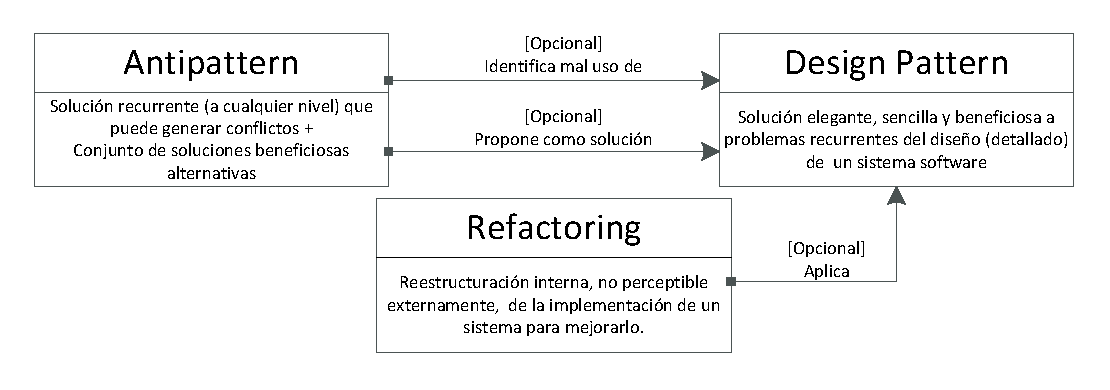
\includegraphics[width=11cm,keepaspectratio=true]{images/antipatterns/antipatternSchema05.eps}}}
%    \only<7>{
%    \rput[lt](0,-1.5){
%        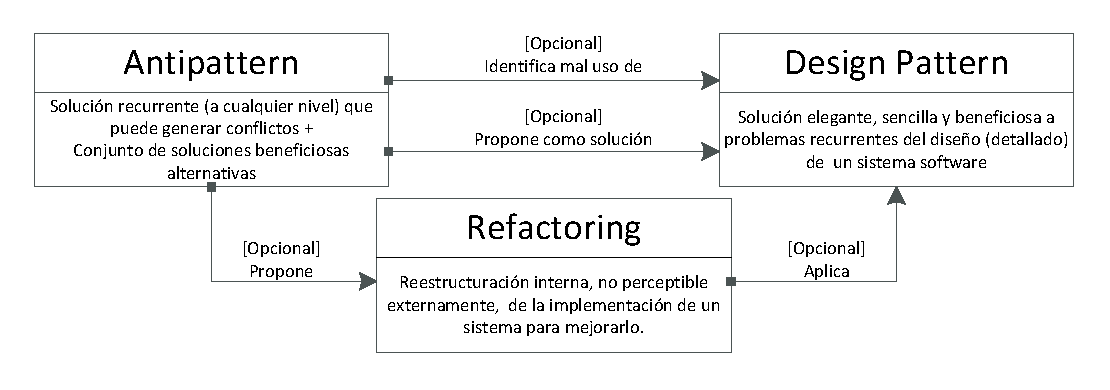
\includegraphics[width=11cm,keepaspectratio=true]{images/antipatterns/antipatternSchema06.eps}}}
%\end{frame}
%
%\begin{frame}[c]
%	\frametitle{Origen de los Antipatrones}
%    \begin{enumerate}[<+->]
%        \item Prisas.     % Mala calidad
%        \item Apatía.     % Para qué
%        \item Estrechez de miras. % No utilizar nuevas y probadas soluciones
%        \item Pereza.     % Confiar en ya se hará con la herramienta
%        \item Avaricia.   % Sistema excesivamente complejo
%        \item Ignorancia. % Pereza intelectual.
%        \item Orgullo.    % stdio está mal.
%    \end{enumerate}
%\end{frame}

\subsection{Spaghetti Code}

\begin{frame}[c]
	\frametitle{Spaghetti Code}
    \begin{block}{Spaghetti Code}
        El código creada tiene una muy pobre estructura. Dicho código suele ser bastante
        monolítico o dependencias exóticas entre métodos y objetos. En general,  resulta difícil de entender, actualizar, mantener y reutilizar (\href{http://imgs.xkcd.com/comics/goto.png}{ejemplo})).
    \end{block}
\end{frame}

\begin{frame}[c]
	\frametitle{Síntomas de Spaghetti Code}
    \begin{enumerate}[<+->]
        \item Métodos excesivamente largos (más de un palmo).
        \item Dependencias no naturales entre objetos.
        \item Métodos con pocos o ningún parámetros.
        \item Propiedades y atributos utilizados como variables globales.
        \item Flujo de ejecución difícil de seguir y predecir.
        \item Estructuras de decisión altamente ramificadas (\emph{if} infernal).
        \item Código difícil de modificar.
    \end{enumerate}
\end{frame}

\begin{frame}[c]
	\frametitle{Causas de Spaghetti Code}
    \begin{enumerate}[<+->]
        \item Malos hábitos de programación.
        \item Falta de encapsulamiento.
        \item Falta de una adecuada descomposición.
        \item Abuso de copiar y pegar.
        \item Abuso de observadores y similares.
        \item Abuso de abstracciones y polimorfismo.
        \item Abuso de inyección de dependencias.
    \end{enumerate}
\end{frame}

\begin{frame}[c]
    \frametitle{Soluciones al Spaghetti Code}
    \begin{enumerate}[<+->]
        \item Aplicación de refactorizaciones como \emph{Extract Method}.
        \item Dividir clases grandes en dos o más clases.
        \item Aplicación de patrones de diseño como \emph{Strategy}, \emph{State}, \emph{TemplateMethod}, \emph{Visitor} o \emph{Abstract Factory}.
    \end{enumerate}
\end{frame}

\subsection{Copy \& Paste Programming}

\begin{frame}
	\frametitle{Copy \& Paste Programming}
	\begin{block}{Copy \& Paste Programming}
		Un trozo de código cuasi-idéntico aparece en diversos lugares del código de un sistema software.
	\end{block}
\end{frame}

\begin{frame}[c]
    \frametitle{Síntomas del Copy \& Paste Programming}
    \begin{enumerate}[<+->]
        \item La solución de un \emph{bug} requiere modificaciones similares en diversas partes del código.
        \item El código es artificialmente largo y repetitivo.
        \item La forma de reutilización de ciertos trozos de código se basa en \emph{copiar y pegar}.
    \end{enumerate}
\end{frame}

\begin{frame}[c]
	\frametitle{Causas del Copy \& Paste Programming}
    \begin{enumerate} [<+->]
        \item Utilización de Copia y Pega como instrumento de reutilización.
        \item Falta de tiempo para crear los mecanismos de reutilización adecuados.
        \item Falta de habilidad técnicas para crear elementos sw reutilizables.
        \item Ausencia de recompensas a nivel corporativo por los esfuerzos realizados para crear elementos reutilizables.
        \item Falta de estabilidad en los equipos de trabajo.
        \item Exceso de orgullo.
    \end{enumerate}
\end{frame}

\begin{frame}[c]
    \frametitle{Soluciones al Copy \& Paste Programming}
    \begin{enumerate}[<+->]
        \item Aplicación de refactorizaciones como \emph{Extract Method} o \emph{Pull-Up Method}.
        \item Utilizar polimorfismo.
        \item Utilizar genéricos.
        \item Utilizar funciones lambda.
        \item Utilizar metadatos y parametrización externa.
        \item Utilizar plantillas de generación de código.
    \end{enumerate}
\end{frame}

\subsection{Lava Flow}

\begin{frame}
	\frametitle{Lava Flow}
	\begin{block}{Lava Flow}
        Un conjunto de código creado durante una fase inicial de concepción de una parte de un proyecto sw pasa a formar parte de dicho proyecto sw. Pasado un cierto tiempo, la mayoría de los desarrolladores ni entiende la utilidad o propósito de dicho trozo de código ni se atreve a modificarlo.
	\end{block}
\end{frame}

\begin{frame}[c]
    \frametitle{Síntomas del Lava Flow}
    \begin{enumerate}[<+->]
        \item Porciones de código sin justificación aparente dentro de un proyecto.
        \item Porciones de código aparentemente críticas sin documentar.
        \item Porciones de código comentadas dentro de clases que están en producción.
        \item Porciones de código comentadas como \emph{To be reviewed} o \emph{To be replaced}.
        \item Existencia de porciones de código muerto.
        \item Existencia de versiones de clases obsoletas.
    \end{enumerate}
\end{frame}

\begin{frame}[c]
	\frametitle{Causas del Lava Flow}
    \begin{enumerate} [<+->]
        \item Utilización de código de prototipado o exploratorio como código de producción sin limpieza previo.
        \item Código escrito sin adherirse a las normas de la organización.
        \item Distribución de código sin control de calidad previo.
        \item Inexistencia de políticas de gestión de la configuración.
        \item Inexistencia de una arquitectura sw.
        \item Requisitos poco definidos y muy cambiantes.
        \item Facilidad para descartar código sin borrarlo.
    \end{enumerate}
\end{frame}

\begin{frame}[c]
    \frametitle{Soluciones al Lava Flow}
    \begin{enumerate}[<+->]
        \item Refactorizaciones extensivas y por tanto caras.
        \item Políticas claras de gestión de la configuración.
        \item Existencia de una arquitectura bien definida.
        \item Existencia de unas reglas arquitectónicas bien definidas.
        \item Políticas claras de control de la calidad.
    \end{enumerate}
\end{frame}

\subsection{La Cosa}

\begin{frame}
	\frametitle{La Cosa}
	\begin{block}{La Cosa (The Blob)}
        Clase principal o central de una aplicación que se encarga de coordinar el resto de clases, las cuales básicamente encapsulan datos.
	\end{block}
\end{frame}

\begin{frame}[c]
    \frametitle{Síntomas de La Cosa}
    \begin{enumerate}[<+->]
        \item Clases con muchas funciones y propiedades.
        \item Clases con una baja cohesión (LCOM4 alto).
        \item Clases controladores de numerosos eventos.
        \item Clases con excesivas dependencias.
        \item Clases con un alto consumo de memoria.
    \end{enumerate}
\end{frame}

\begin{frame}[c]
	\frametitle{Causas de La Cosa}
    \begin{enumerate} [<+->]
        \item Falta de habilidades relacionadas con la orientación a objetos.
        \item Ausencia de una arquitectura software.
        \item Ausencia de control de calidad.
        \item Pereza a la hora de asignar responsabilidades.
    \end{enumerate}
\end{frame}

\begin{frame}[c]
    \frametitle{Soluciones a La Cosa}
    \begin{enumerate}[<+->]
        \item Agrupar métodos y atributos en bloques fuertemente cohesionados.
        \item Asignar estos conjuntos de métodos y atributos a clases.
        \item Eliminar asociaciones inútiles.
        \item Aplicar patrones para manejar estados y comportamientos variables.
    \end{enumerate}
\end{frame}

%
%\subsection{Singletonitis}
%
%\begin{frame}
%	\frametitle{Singletonitis}
%	\begin{block}{Escenario}
%		Un programador abusa del patrón \emph{Singleton}, el cual usa principalmente para evitar tener que mantener referencias entre objetos o pasar parámetros.
%	\end{block}
%	\uncover<2->{
%		\begin{block}{Problemas}
%			\begin{enumerate}
%				\item<2-> Todos los asociados con las variables globales.
%				\item<3-> No se pueden crear varias instancias de clases que no tienen \alert{porqué tener una instancia única}.
%			\end{enumerate}
%		\end{block}
%	}
%	\uncover<4->{
%		\begin{block}{Solución}
%			No usar el patrón \emph{singleton} cuando no tiene sentido usarlo.
%		\end{block}
%	}
%\end{frame}

\section{Sumario y Referencias}
%
%\subsection{Sumario}
%
%\begin{frame}[c]
%	\frametitle{¿Qué tengo que saber de todo esto?}
%	\begin{enumerate}
%		\item<1-> Comprender el concepto de patrón.
%		\item<2-> \alert<8>{Saber aplicar el catálogo de patrones GoF}.
%		\item<3-> \alert<8>{Saber aplicar los patrones \emph{tipo} y \emph{mixin}}.
%		\item<4-> Comprender el concepto de antipatrón.
%		\item<5-> Saber aplicar los antipatrones \emph{programación basada en copiar y pegar} y \emph{singletonitis}.
%		\item<6-> Comprender el concepto de refactorización.
%		\item<7-> Saber aplicar las refactorizaciones \emph{pull up method}, \emph{move method}, \emph{add parameter}, \emph{move field}, \emph{rename method} y \emph{rename field}.
%	\end{enumerate}
%\end{frame}
%
\subsection{Referencias}

\begin{frame}
	\frametitle{Referencias}
	\bibliographystyle{apalike}
	\bibliography{disenhoSoftware}
\end{frame}

\end{document}
